\documentclass[article,12pt,english, a4paper, oneside, onecolumn, openany]{memoir}
\usepackage{fix-cm,fixltx2e}
\usepackage{babel}  % babel: Hyphenation patterns and language specific strings
\usepackage{varioref}
\usepackage[colorlinks,linkcolor=black,urlcolor=black,citecolor=black]{hyperref}
\usepackage[latin1]{inputenc}
\usepackage{graphicx}
\usepackage{listings}
\usepackage[square,numbers]{natbib}
\usepackage{url}
\usepackage{pslatex}
\usepackage{pdfpages}
\usepackage{placeins} % gives me FloatBarrier
%Forhindrer floats i at flyde ind i n�ste afsnit
\let\oldsection=\section % gemmer den gamle definition
\renewcommand\section{\FloatBarrier\oldsection}

\makeatletter
\renewcommand\fps@figure{htbp} % Force figure placement
\renewcommand\fps@table{htbp}
\makeatother

% setup captions
\hangcaption
\changecaptionwidth
\captionwidth{9cm}

\usepackage[margin=2.5cm]{geometry}
\linespread{1.166667}

\pagestyle{plain}
\title{Final Assignment\\\textbf{Software Architcture Analysis Report}}
\author{S�ren B. Vrist\\\url{sbvr@itu.dk}}
\begin{document}
\frontmatter
\maketitle
\tableofcontents
\newpage
\mainmatter
\chapter{Introduction}
This report will do an architechture analysis of the JCommSy software as
provided by \url{http://www.commsy.net}. The software provides a collabrative
community system for project work. 
\begin{itemize}
  \item How the system looks like(4+1 view)
  \item introduction of scope
\end{itemize}

\chapter{Theoretical foundation}
Papers:
\begin{itemize}
  \item \citep{4plus1}
  \item \citep{gqm}
  \item \citep{gqm84}
\end{itemize}
\ldots

\chapter{Intended architechture}
The intended architechture as given by the project is illustrated in figure
\ref{fig:intarch}.

\chapter{Analysis}
\begin{itemize}
  \item Metrics
  \item Oberservations
\end{itemize}

\chapter{Refactoring}
\begin{itemize}
  \item identify problems (>2)
  \item Suggest actions
  \item Argue with business constraints
  \item Refactoring plan (1-2)
\end{itemize}

\chapter{Conclusion}
\ldots

\backmatter
\listoftables
%\listoffigures

\bibliography{biblio}
\bibliographystyle{alphaurl}
\clearpage
\appendix
\chapter{Appendix}

\chapter{Figures}
\section{Architechture image}
\begin{figure}
  \centering
  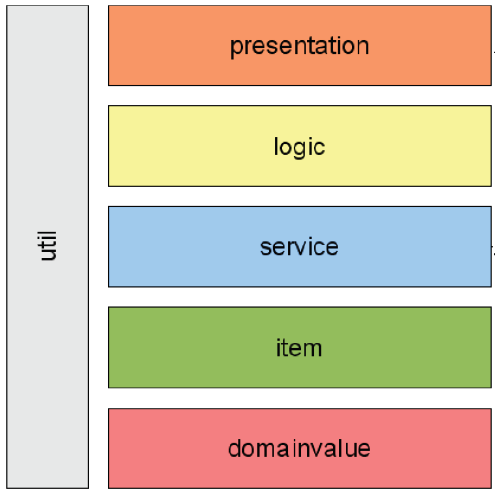
\includegraphics[width=11cm]{arch}
  \caption{The given overview of JCommSy architechture}\label{fig:intarch}
\end{figure}
\end{document}
